%%--------------------------------------------
%% Inverse Dynamics
%%--------------------------------------------


Without external contacts, the inverse dynamics of a robot with $m$ degrees of freedom can be generally described by 
%
\begin{align}
  \torques = \underbrace{\inertiaMatrix\ddq + \Hmatrix}_{\torques_\text{RBD}} + \epsilon\,(\q,\dq,\ddq) \,,
  \label{eq:tau_nocontact}
\end{align}
%
where $\q\in \R^{m}$, $\dq \in \R^{m}$ and $\ddq \in \R^{m}$ are the joint positions, velocities and accelerations, respectively, $\inertiaMatrix \in \R^{m \times m}$ is the inertia matrix, and $\Hmatrix \in \R^{m \times m}$ is the matrix combining the contributions from Coriolis and centripetal, friction (viscous and static) and gravity forces:
%
\begin{align}
	\Hmatrix = \coriolis(\q,\dq)\dq + \gravityMatrixNo(\q) + F_v \dq + F_s \,\text{sgn}(\dq) \,.
\end{align}
%
The term $\epsilon(\q,\dq,\ddq)$ in \eq\eqref{eq:tau_nocontact} captures the errors of the model,
such as unmodeled dynamics (e.g., elasticities and Stribeck friction),
inaccuracies in the dynamic parameters (e.g., masses, inertia),
vibrations, couplings, and sensor noise. 

In presence of a set $\mathcal{C}=\{c_1 \ldots c_n\}$ of contacts $c_i$ between the robot and the environment, \eq\eqref{eq:tau_nocontact} becomes
%
\begin{align}
	\torques = \underbrace{\inertiaMatrix\ddq + \Hmatrix}_{\torques_\text{RBD}} + \epsilon(\q,\dq,\ddq) + \color{darkgreen}{\sum_{c_i \in\mathcal{C}} {\jacobian\T_{c_i}(\q)}\, \extForces_i} \,\color{black}{,}
	\label{eq:tau_contact}
\end{align}
%
where the last term accounts for the effect of the external wrenches
(forces and moments) $\extForces_i$ applied at the
contact location $c_i$, and $\jacobian_{c_i}(\q)$  is the contact Jacobian\footnote{The contact location $c_i$ is not necessarily fixed, as the contacts may occur on the whole robotic structure and not exclusively at the end-effectors. 
In such a case, the contact location, if not known a priori, must be estimated, typically through distributed tactile sensors.
To compute the contact Jacobian, we need the position of the contact point with respect to the reference frame of the link~\cite{Fumagalli2012}. 
Such a knowledge requires a kinematic calibration of the skin, as explained in~\cite{DelPrete2011}.}.
%\todo[inline]{What exactly is a contact location? What coordinate
%  system? Explain these things}
%


%%=================================================================================================

\subsection{Classical Model-based Approaches for Computing the Inverse Dynamics}

	Classical approaches for computing $\torques$ or $\torques_\text{RBD}$ rely on the dynamics model with known or identified kinematics and dynamics parameters~\cite{Ivaldi2011}. 
   	The torques $\torques_\text{RBD} = \inertiaMatrix\ddq + \Hmatrix$ can be computed analytically through the rigid body dynamics model of the robot, a standard parametric description of the robot~\cite{Featherstone2008}. 
   	Conversely, the term $\epsilon(\q,\dq,\ddq)$ is often neglected, or implicitly taken into account by considering a perturbation in the dynamics parameters of $\torques_\text{RBD}$, which need to be identified accurately.




      % \todo[inline]{ Fix this.
      % 	The inverse dynamics does not have discontinuities. 
      % 	However, the measurement noise is not homogeneous in the system, as measurement during contacts is much noisier than for free movements.
      % 	Hence, the use of heteroscedastic models is well suited to the task and might provide huge benefits compared to standard homoscedastic models.}


      %==> now we start with classical methods and robot identification.. etc etc
      %The accuracy of the robot dynamics model therefore depends on the accuracy of its dynamics parameters.

	Although the parameter identification for industrial robots is relatively easy with exciting trajectories~\cite{Pedrocchi2014}, the procedure for floating-base robots, such as humanoids, is not straightforward because of two main issues: 
      The first issue is the generation of sufficiently large accelerations for the identification while maintaining the robot balance and the control of contacts. 
      This issue was well explained by Yamane~\cite{yamane2011}, who proposed a technique to identify the mass and the local COM of the links in a humanoid robot with fixed feet at the ground and slow joint trajectories. 
      The second issue is the measurement of the external forces $\extForces_i$ exerted on the robot.
      Note that it may not be straightforward to measure the external forces~$\extForces_i$, as it is not possible to cover the robot body with 6-axis force/torque sensors to measure the force exerted on every possible contact location $c_i$. Usually, such sensors are big, heavy and expensive, thus they are carefully placed where the external forces are critical for the main tasks, for example at the end-effectors for manipulation and at the feet for balancing.
      In such a case, it is possible to identify the dynamics parameters while balancing and walking without additional contacts~\cite{Ogawa2014}.
      When force/torque sensors are placed proximally, such as in the \robot{} arms~\cite{Fumagalli2012}, some of the dynamics parameters can be identified, but in absence of contacts~\cite{Traversaro2013}.

      When multiple contacts are exerted on the robot structure at locations other than the classical end-effectors, it is still possible to compute a precise inverse dynamics model, but this requires both pervasive joint torque sensing, such as in \textit{Toro}~\cite{Ogawa2014}, and additional force/torque and tactile sensing, such as in \robot{}~\cite{Ivaldi2011}.
      Moreover, it requires the precise knowledge of the contact locations detected by the tactile sensors, which necessitates a spatial calibration of the skin~\cite{DelPrete2011}. 
      This procedure is prone to errors, and it has been shown that small errors in the kinematics calibration of the taxels (i.e., the tactile units) can induce non-negligible errors in the estimation of the contact forces~\cite{DelPrete2012}.

      Overall, these approaches have three main limitations: 
      First, since they are model-based, it is difficult to add details about couplings, elasticity, friction and other nonlinear dynamics, which would be required for high accuracy; 
      Second, the performance of the data-driven identification strongly depends on the experimental setting (with/without contacts) and the exciting trajectories~\cite{Pedrocchi2014}; 
      Third, they make strong assumptions in order to handle contacts.

      %An alternative and appealing approach is to learn the dynamics model through machine learning techniques~\cite{Nguyen-Tuong2008,Vijayakumar2000}. 
      %The main advantage of this approach has been clearly stated in \cite{Nguyen-Tuong2011}, where the authors showed that a learned dynamics could improve the performance of inverse dynamic control.

%%=================================================================================================


\subsection{Learning the Inverse Dynamics}

        An alternative and appealing approach to model-based dynamics computation is to use machine learning methods to learn the dynamics model of a robot~\cite{Nguyen-Tuong2008,Vijayakumar2000,Deisenroth2012}. 
        Without the need to compensate for inaccurate dynamics parameters and accumulated errors, a learned dynamics model can improve the tracking and control performance of a robot, as shown in~\cite{Nguyen-Tuong2011} for an industrial manipulator.
        The clear advantage of learning the inverse dynamics is that we can overcome the limitations of the aforementioned approaches: difficulty in modeling complex nonlinear dynamics, impossibility to generate suitable exciting trajectories, restrictive assumptions regarding contacts and sensors, prior accurate kinematics calibration of the tactile sensors.
        %\todo[inline]{Unclear how learning overcomes these limitations}
        %Several machine learning techniques have been applied to the problem of learning inverse dynamics, for example GP~\cite{???}, LGP~\cite{Nguyen-Tuong2008} and LWPR~\cite{Vijayakumar2000}.
        %The better performance comes from the fact that we can easily learn unmodelled dynamics and the accumulated errors due to the inaccurate dynamics parameters. 
        %For example, in \cite{Nguyen-Tuong2011} a learned dynamics could improve tracking performance in computed torque control for an industrial manipulator.

        %However, to the best of our knowledge there are no examples in the literature where multiple contacts are also learned. 
        %Prior works on learning or improving the inverse dynamics model lack a fundamental aspect: the inclusion of multiple contact dynamics in the model.
        The inclusion of multiple contact models in the dynamics highlights two main problems:
        %There are two main problems.
        First, switching from a no-contact model to a contact-model requires to observe the system state and to model a discontinuous function~\cite{Toussaint2005}. 
        Second, switching between different contacts $c_i \in\mathcal{C}$ must be properly handled. %and to combine multiple ones simultaneously: that is dealing with a multitude of  $c_i \in\mathcal{C}$.\todo{unclear}

        %
        Here, we provide a formulation to this problem, and we show that it is possible to learn the inverse dynamics model of the robot by means of proximal force/torque measurements~$\ftsForces$ and distributed tactile sensors~$\skinInput$ such that:
        %
        \begin{align}
        	\torques = \torques_\text{IDM}(\q,\dq,\ddq,\skinInput,\ftsForces) \,.
            \label{eq:torques}
        \end{align}
        %

        % The benefit of such a model are many. 
        % It only introduces an additional sensor measurement $\skinInput$, which provides the information about the contact location and a measure of the applied force on the taxel. 
        % Tactile sensors are cheaper and lighter than force/torque sensors: with such a model, it can be possible to apply torque control to robotic manipulators in presence of dynamics contacts in locations other than the end-effector, which makes it possible to control physical interaction with an evolving environment or humans.
        This solution enables a fast and accurate prediction of joint torques in situations when the robot is in contact with no, one or even multiple simultaneous contacts, detected by a tactile skin.
        The estimation does not rely on dynamic parameters or parametric models, but it is completely data driven: Tactile sensors provide information about the contact locations (without requiring a spatially calibrated model of the skin~\cite{DelPrete2011}), while force/torque sensors provide information about the wrenches perceived by the robotic structure.
        %; joint torque sensors, here, provide the ground truth measurements.\footnote{If robots are not equipped with joint torque sensors, in most cases it is possible to compute the joint torque through the motor current.}
        %Our experiments are carried out on the humanoid robot iCub \cite{Natale2013}.

        We detail our proposed model and its learning procedure in the following section.

%
\begin{figure}[t]
  \centering
  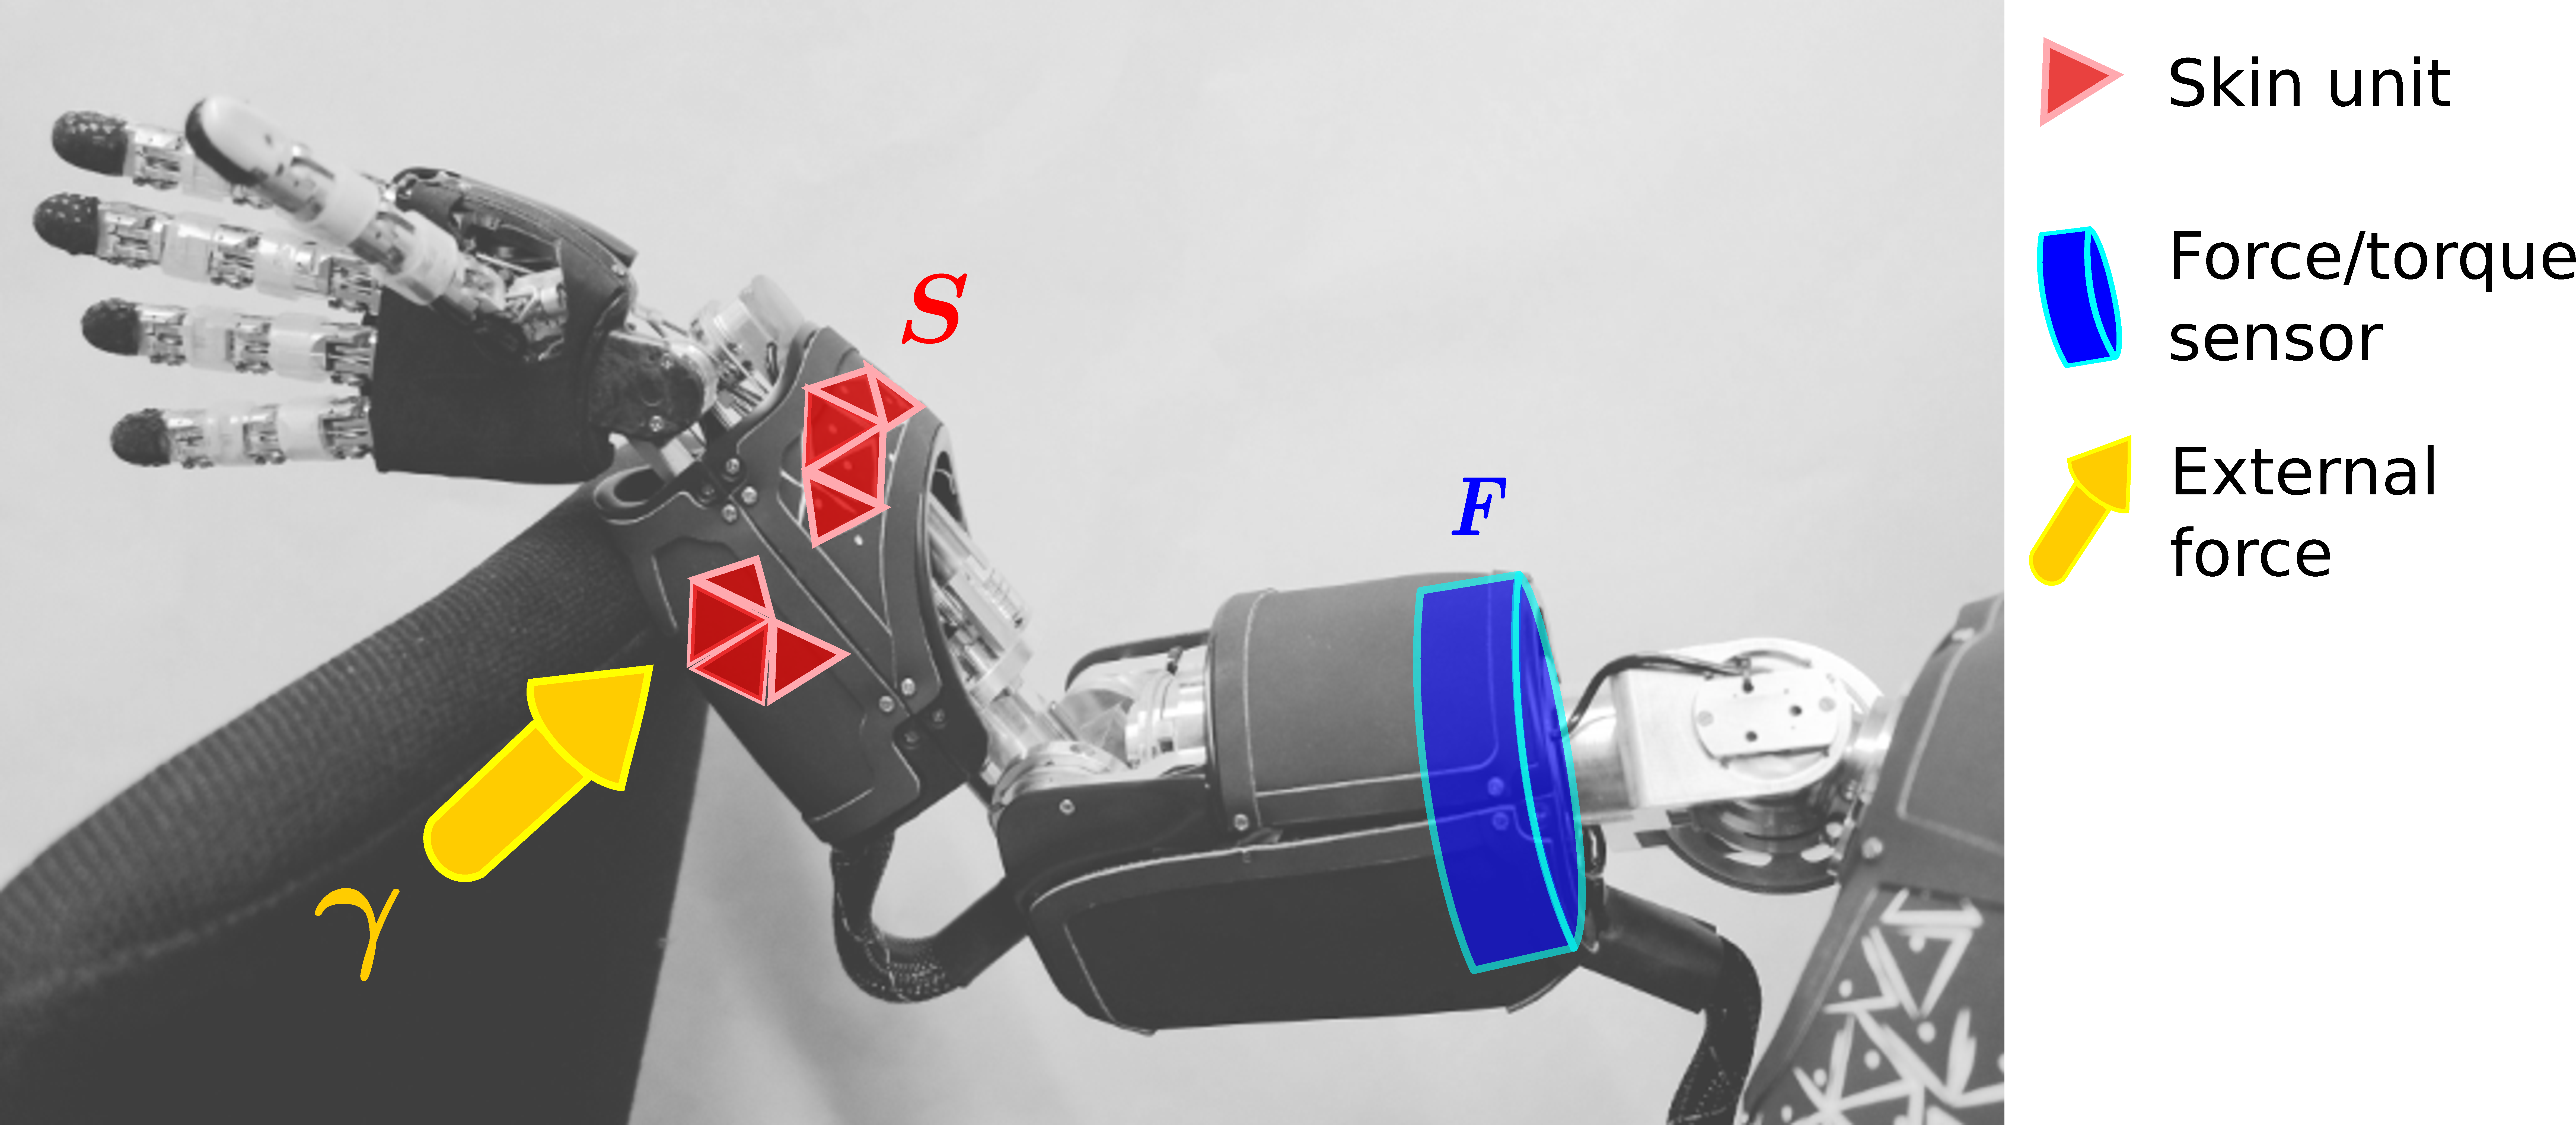
\includegraphics[width=.5\columnwidth]{robertoIROS/fig/concept_gray}		
  \caption{Illustration of the force/torque and tactile sensors involved during a contact of the robot arm with the environment.}
  \label{fig:concept}
\end{figure}
%
